\documentclass{article}
% translate with >> pdflatex -shell-escape <file>

% This file is used as unit test for pgfplots, copyright by Christian Feuersaenger.
% 
% See
%   http://pgfplots.sourceforge.net/pgfplots.pdf
% for pgfplots.
%
% Any required input files (for <plot table> or <plot file> or the table package) can be downloaded
% at
% http://www.ctan.org/tex-archive/graphics/pgf/contrib/pgfplots/doc/latex/
% and
% http://www.ctan.org/tex-archive/graphics/pgf/contrib/pgfplots/doc/latex/plotdata/

\usepackage{pgfplots}
\pgfplotsset{compat=newest}

\pagestyle{empty}

\begin{document}


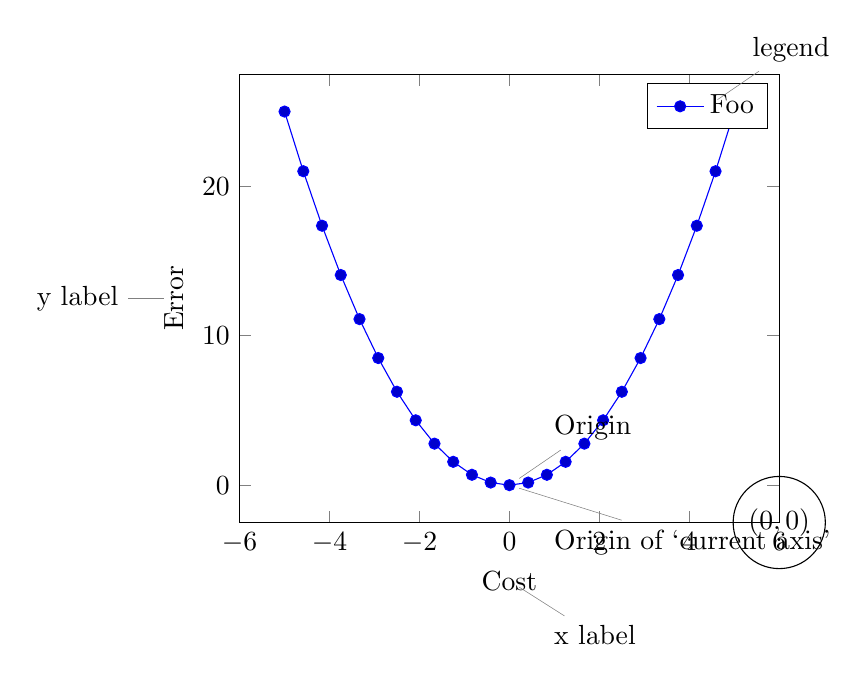
\begin{tikzpicture}[baseline]%
	\node[circle,draw=black] at (0,0) {$(0,0)$};
	\begin{axis}[
		anchor=south east,
		name=firstplot,
		xlabel=Cost,
		ylabel=Error,
		y label style={name=myylabel},
		x label style={name=myxlabel},
		legend style={name=mylegend,
			row 1 column 2/.style={blue,name=firstentry}% doesn't work!
		}
	]
	\addplot (\x,\x^2);
	\legend{Foo}
	\end{axis}

	\node[pin=45:legend] at (mylegend.center) {};
	\node[pin=-45:x label] at (myxlabel.center) {};
	\node[pin=180:y label] at (myylabel.center) {};

	\node[pin=45:Origin] at (firstplot.origin) {};
	\node[pin=-45:Origin of `current axis'] at (current axis.origin) {};
\end{tikzpicture}
\end{document}
